\section{Methods}
\label{sec:Methods}

The data of the vehicular experiment was gathered at the intersection of Universitätsallee and Otto-Hahn-Allee respectively Bibliothekstraße in Bremen, Germany. There are 14 possible paths for the vehicles,
which were split between the two group members to observe and manually collect. The first group member observed directions 1 to 7, whereas the second group member observed directions 7 to 14. Figure \ref{fig:intersection} shows a sketch of the intersection including all numerated paths, the observing point, as well as the tram rails which are assigned to directions 1 and 14. 
\begin{figure}[hbtp]
\centering
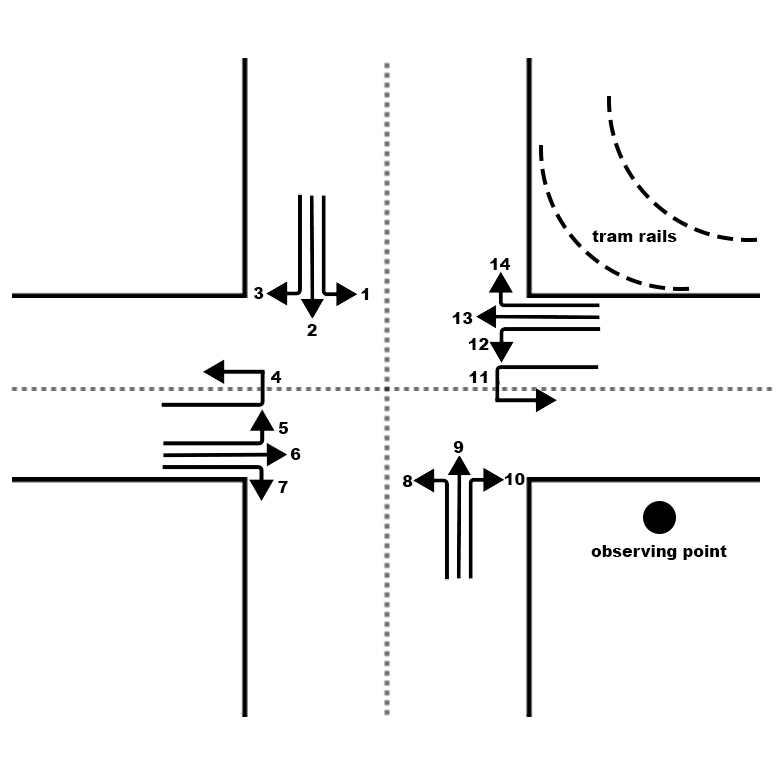
\includegraphics[width=.9\linewidth]{intersection.jpg}
\caption{Sketch of the intersection Universitätsallee and Otto-Hahn-Allee in Bremen, Germany}
\label{fig:intersection}
\end{figure}

A total of four separate experiments were conducted, with each experiment containing four individual measurements for a time period of 10 minutes. The date, time, and temperature of each experiment is shown in Table \ref{tbl:experiments}. Starting at the predetermined time, a stop watch was started for exactly 10 minutes. After a 5 minute break, another measurement was conducted identically.
\begin{center}
\begin{tabular}{ |p{4.5em}|p{3.5em}|p{7.5em}|p{5.5em}|}
 \hline
 Experiment & Date & Time & Temperature  \\
 \hline
 1 & 30.05.22 & 8:05am - 9:00am & $9^\circ$C - $10^\circ$C \\
 \hline
 2 & 30.05.22 & 9:05am - 10:00am & $11^\circ$C \\
 \hline
  3 & 03.06.22 & 9:05am - 10:00am & $14^\circ$C - $17^\circ$C\\
 \hline
  4 & 10.06.22 & 9:05am - 10:00am & $18^\circ$C - $19^\circ$C \\
 \hline
\end{tabular}
\captionof{table}{Dates, times, and temperatures of each experiment}
\label{tbl:experiments}
\end{center}
~\\
During each measurement the amount of cars taking a certain path and their according timestamp, in minutes and seconds (e.g. 1:21) was noted. Vehicles such as trams, buses and motorcycles were marked separately. Generally, the timestamp was noted when a vehicle crossed the center of the intersection. 
In case that multiple cars take the same path at the same time the number of cars was noted next to the timestamp. This was done on provided data sheets. The data sheets are shown in the appendix. They contain the date, starting time, group number and temperature for each individual 10-minute-measurement in the top left corner.


